% !TeX spellcheck = en_US
\documentclass[11pt,a4paper,oneside,openright]{article}

\usepackage[utf8]{inputenc}
\usepackage[english]{babel}
\usepackage{amsmath}
\usepackage{mathtools}
\usepackage{amsfonts}
\usepackage{amssymb}
\usepackage{listings}  % Required for insertion of code
\usepackage{graphicx} % Required to insert images
\usepackage{textcomp}
\usepackage{enumerate} % Required for enumerate model
\usepackage{gensymb} %Required for degree symbol which is made ^{\circ}
\usepackage{caption} %used to have cool captions
\captionsetup{
	tableposition=top,
	figureposition=bottom,
	font=small,
	format=hang, 
	labelfont=bf}	%caption setup
\usepackage[protrusion=allmath]{microtype} %used to have high quality text formatting
\usepackage{graphicx,subfig,float,wrapfig,rotating,multirow,epstopdf} %high quality tables and images formatting
\usepackage{booktabs,siunitx,array,tabularx} % tables
\usepackage{amsbsy,bm,amsmath} % math

%\usepackage [ Lenny ]{fncychap}
\usepackage{longtable} % Required to put long tables

\lstset{ % Frame for Matlab code
	numbers=left, 
	numberstyle=\small, 
	numbersep=8pt, 
	frame = single, 
	language=Matlab, 
	framexleftmargin=19pt,
	breaklines}

\pagestyle{plain}

\graphicspath{{img/}} % Set graphics directory

\def\permille{\ensuremath{{}^\text{o}\mkern-5mu/\mkern-3mu_\text{oo}}} % Add symbol of per mille
\newcommand{\parallelsum}{\mathbin{\!/\mkern-5mu/\!}} % Fix parallel symbol inclination

%\makeindex

\title{	01NVSOQ -- Advanced Antenna Engineering \\
	\huge {\textsc{Assignment 4: array components}}	}

\begin{document}
\author{Amedeo Bertone (243878)\\Davide Botteon (239595)\\Enrico Maria Renzi (244028)\\
}
\date{January 11, 2018}
\maketitle 		
\tableofcontents

\section{Introduction}

\section{Sections fine tuning}
\paragraph{First T}
First of all we have to better optimize the various part of the beam forming network, and so we started considering the first T junction with the lines routing to the second one. In particular the bending situated between the T junction are introducing a strong discontinuity, which must be considered in the optimization. About the optimization of the bending and the use of the mitered solution for the T junction there are Appendix A and Appendix B that explains the process in details. Below we can see the results obtained in this way.
\begin{figure}[H]
	\centering
	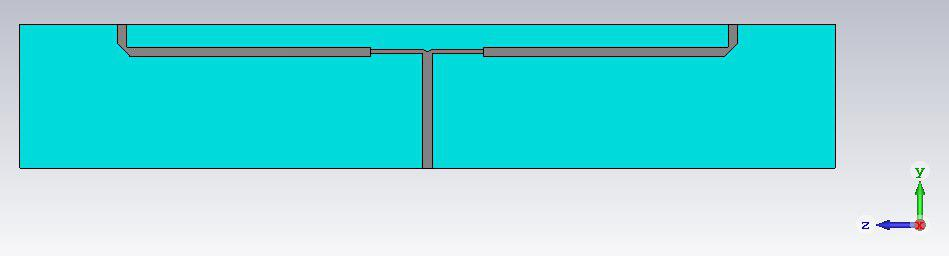
\includegraphics[width=1\linewidth]{fT_struct.jpg}
	\caption{structure of the first T and the branches routing to the second one}
	\label{fT_struct}
\end{figure}
\begin{figure}[H]
	\centering
	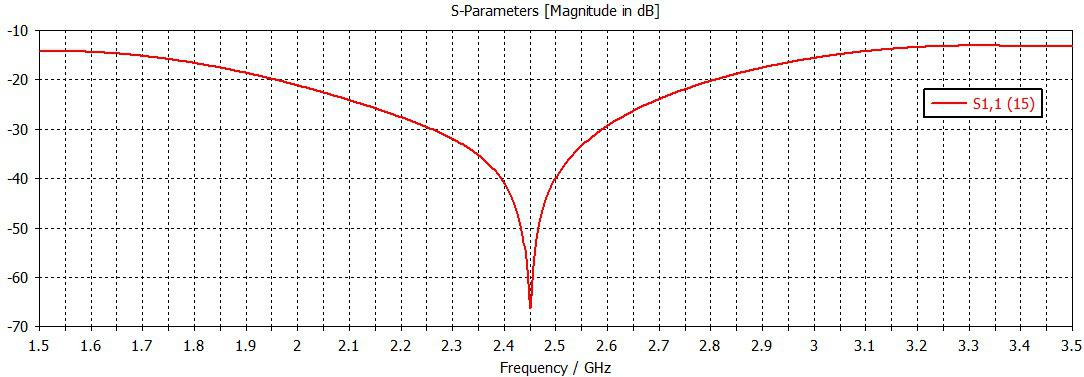
\includegraphics[width=1\linewidth]{fT_fin.jpg}
	\caption{final scattering parameters}
	\label{fT_fin}
\end{figure}

\paragraph{Second T}
Regarding the optimization of the second T junction we used the T designed for the previous assignment and we connect to it the two lines routing to the patches. In this way we control also the contributions due to the discontinuities on all the second part of the beam forming network.
\begin{figure}[H]
	\centering
	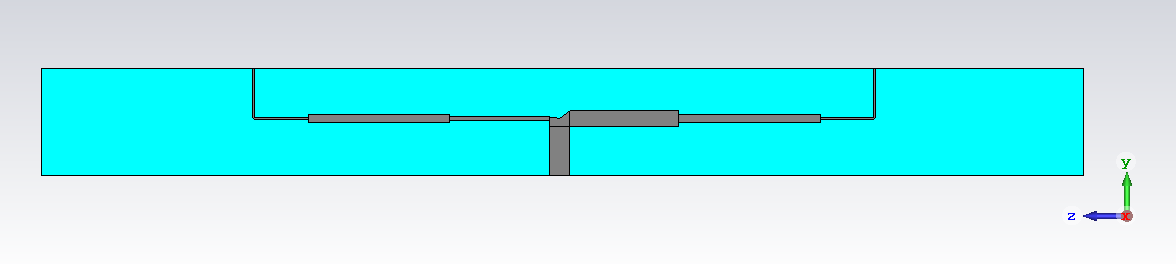
\includegraphics[width=1\linewidth]{sT_struct.png}
	\caption{structure of the second T and the branches routing to the patches}
	\label{sT_struct}
\end{figure}
Simulating this new component we have that the matching is no more on the wanted frequency of $2.45GHz$ but some megahertz higher. In order to make it decrease at first we tried to change the values external to the T junction with a freedom degree, that in particular are the angle and the tapering of the bending (the same process used for the first T, described above). The results varying those values are showed in the graphs below. Notice that in practice the resonance is not moved in both the cases.
\begin{figure}[H]
	\centering
	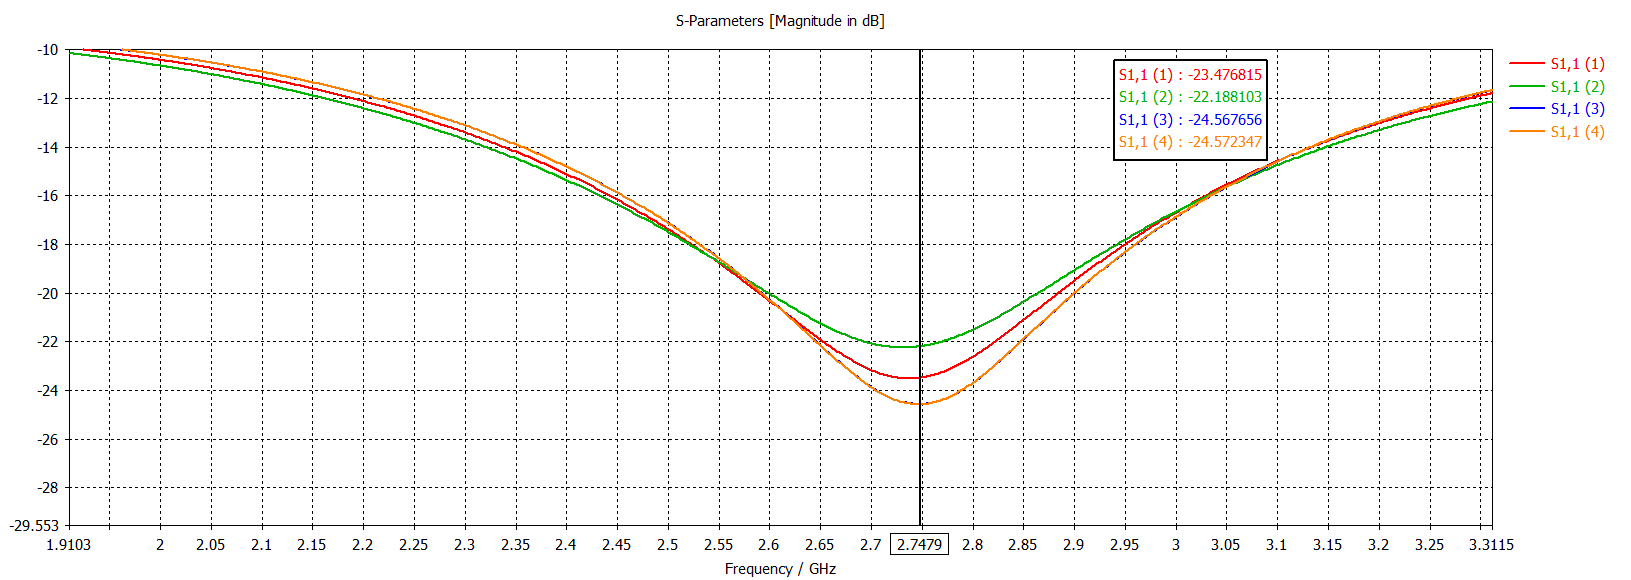
\includegraphics[width=1\linewidth]{sT_1angle.png}
	\caption{s11 with respect to the bend angle}
	\label{sT_1angle}
\end{figure}
\begin{figure}[H]
	\centering
	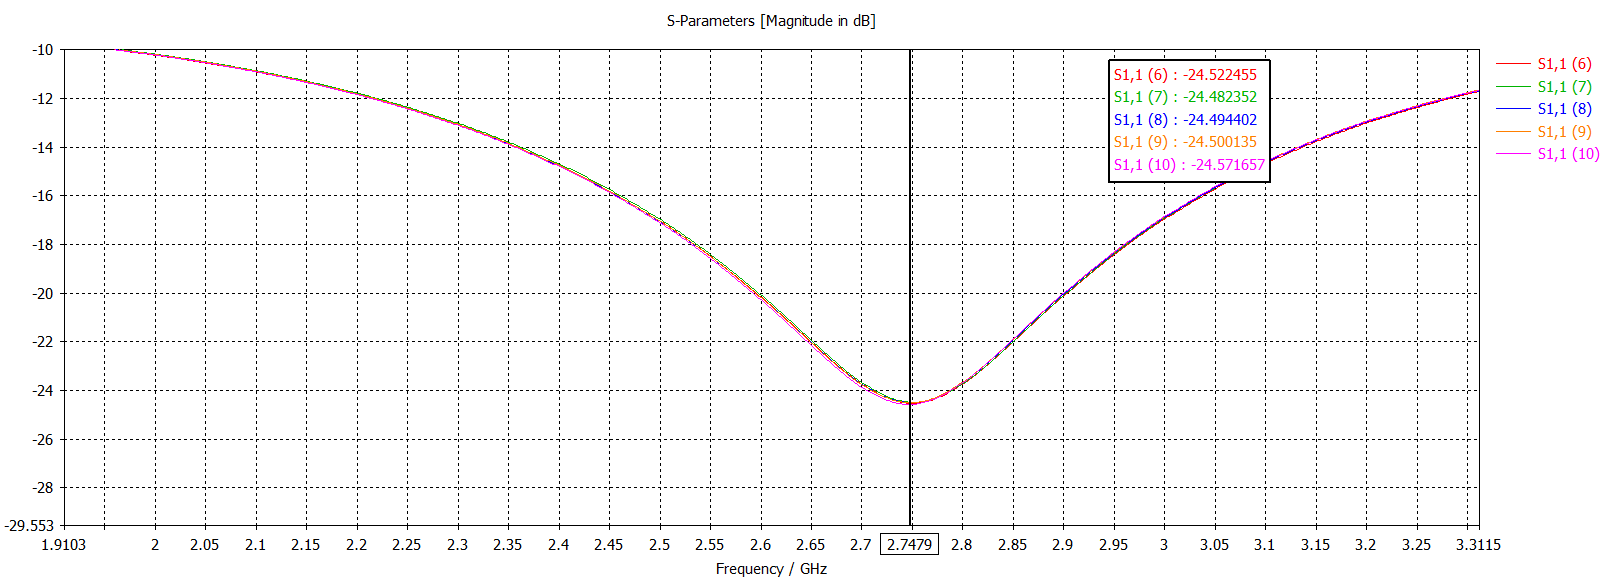
\includegraphics[width=1\linewidth]{sT_1depth.png}
	\caption{s11 with respect to the bend tapering}
	\label{sT_1depth}
\end{figure}
Now we have tried to not modify the T junction parameters, but since this way didn't produce the desired effect we have to change the the $\lambda/4$ impedance transformer's length (changing the other lines' length means changing the tapering). The graphs below shows the values obtained first with simply changing the transformer length and second the also re-using the old optimized value of the single T junction (notice that in the second case the return losses are lower).
%\begin{figure}[H]
%	\centering
%	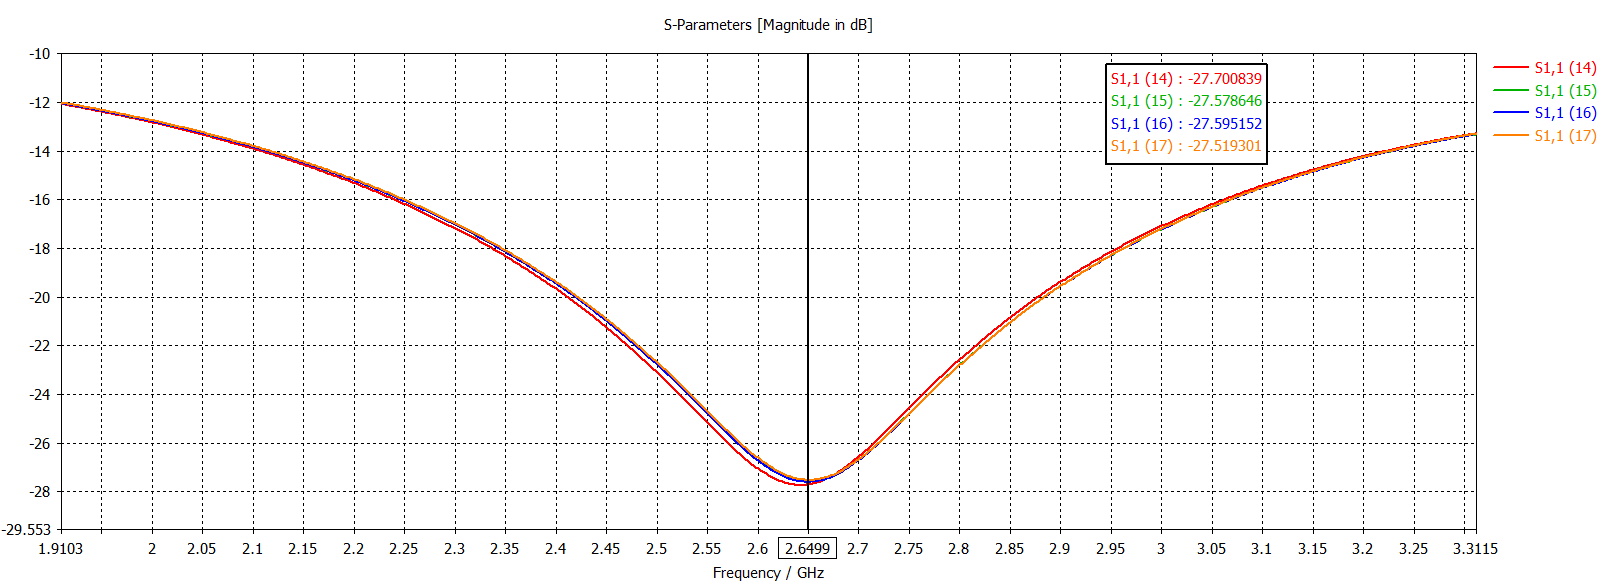
\includegraphics[width=1\linewidth]{sT_2depth.png}
%	\caption{}
%	\label{sT_2depth}
%\end{figure}
\begin{figure}[H]
	\centering
	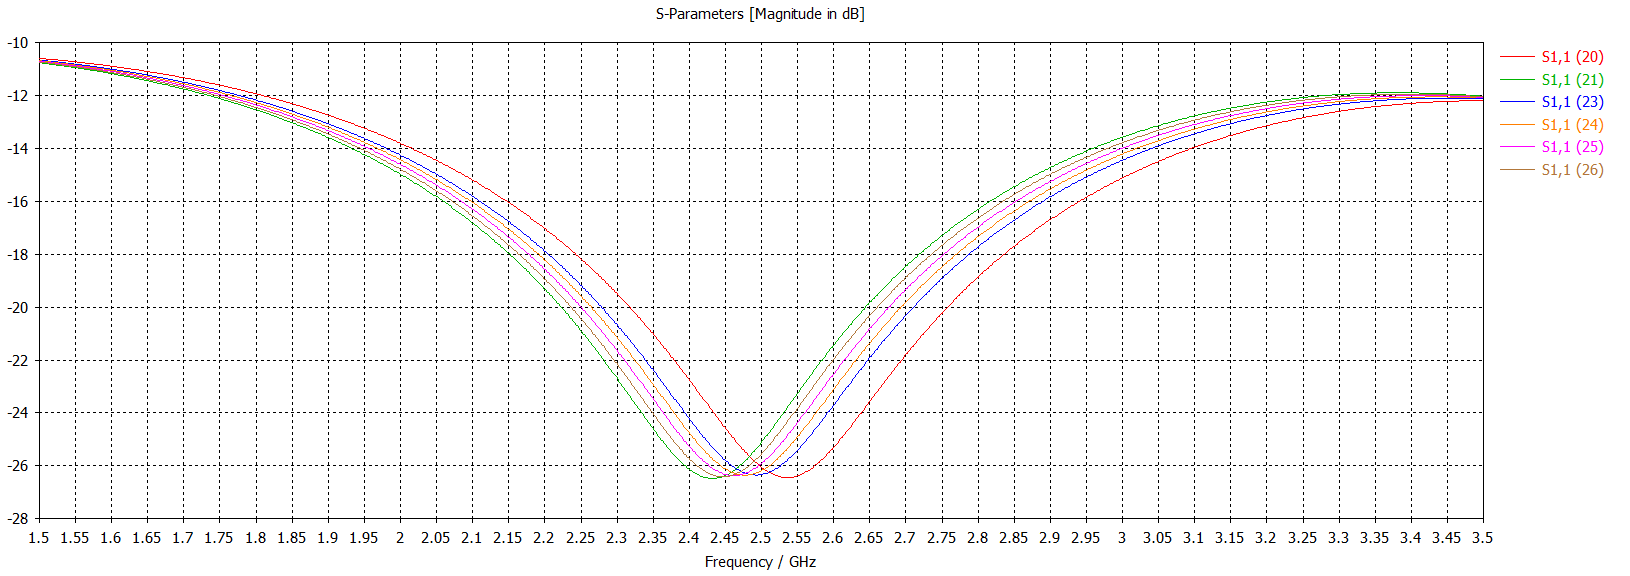
\includegraphics[width=1\linewidth]{sT_2par.png}
	\caption{s11 with respect to the $\lambda/4$ transformer's length}
	\label{sT_2par}
\end{figure}
\begin{figure}[H]
	\centering
	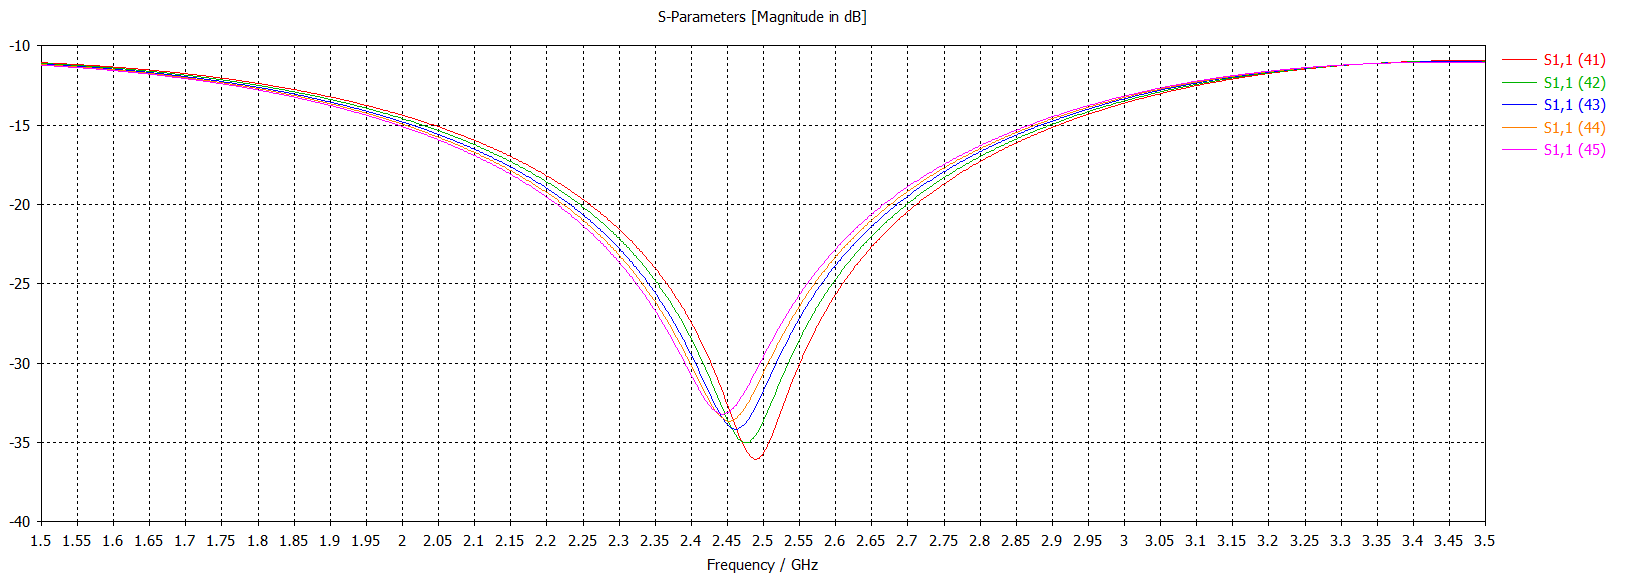
\includegraphics[width=1\linewidth]{sT_3par.png}
	\caption{s11 with respect to the $\lambda/4$ transformer's length -- changed values}
	\label{sT_3par}
\end{figure}
With this final value we reached the desired behavior, so we can use this for composing the complete beam forming network. On the following figure is showed the result, notice that also the $s_{21}$ and the $s_{31}$ have the proper values in order to generate the desired tapering.
\begin{figure}[H]
	\centering
	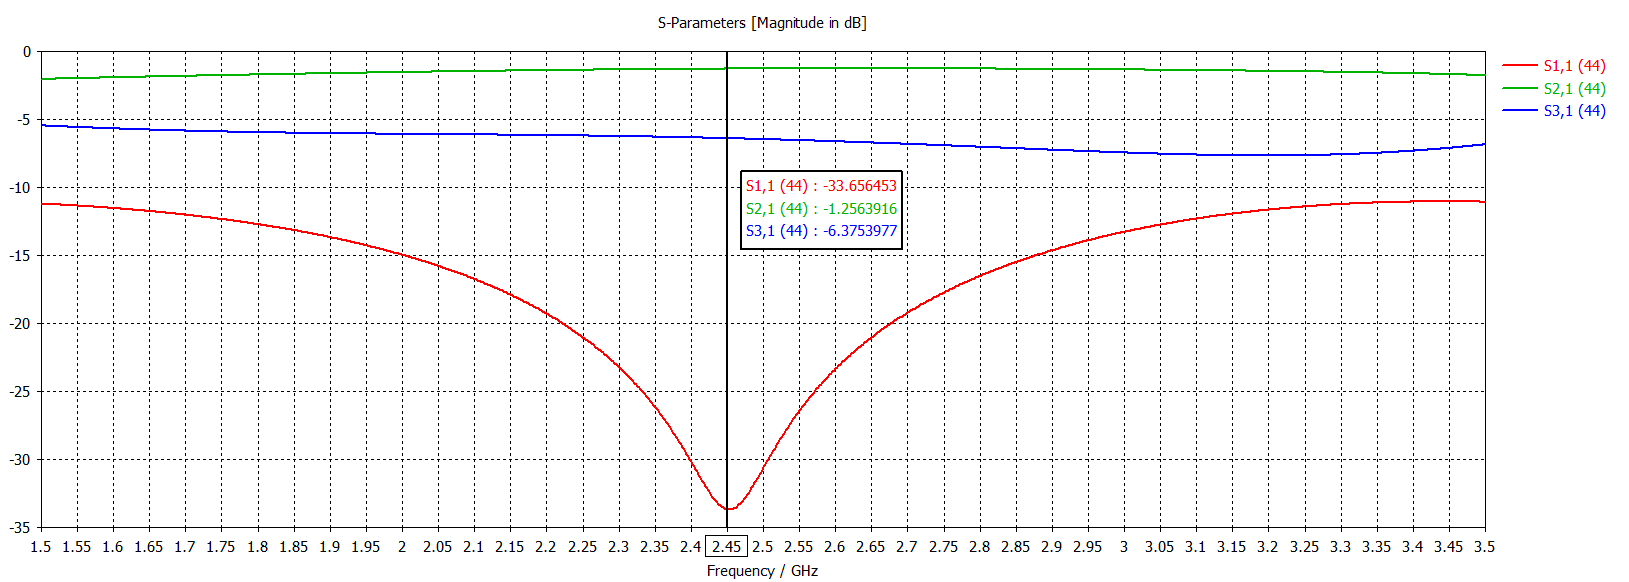
\includegraphics[width=1\linewidth]{sT_fin.png}
	\caption{final scattering parameters}
	\label{sT_fin}
\end{figure}

\section{BFN fine tuning}



\newpage
\section{Full array fine tuning and results}

\begin{figure}[t] 
	\centering
	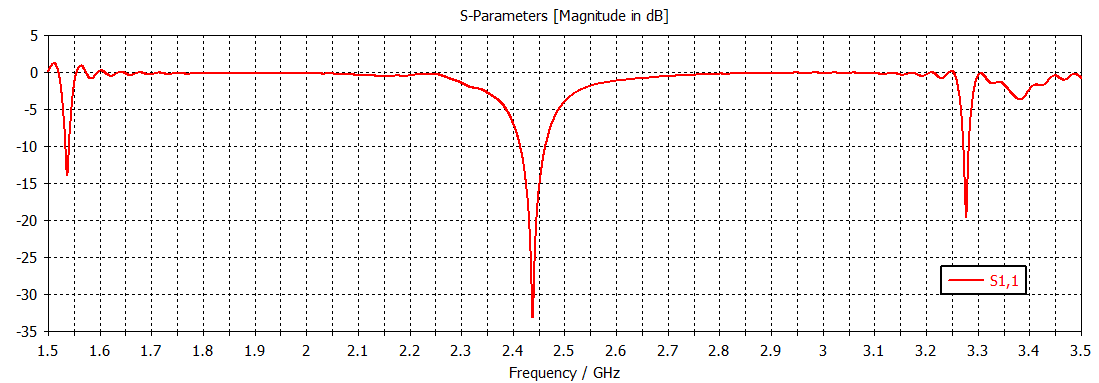
\includegraphics[scale=0.45]{p3_RL}
	\caption{Broadband view for the input reflection coefficient seen from full array input port.}
	\label{fig:p3_scattering}
\end{figure}
Within this last step the tuned BFN and radiating part are connected. The spacing between elements is set to be compliant with the GL limit at the central resonance frequency f\textsubscript{0}=2.45GHz (distance between elements, d=$\leq$88mm). 
Actually what follows mainly concerns the full antenna's radiation pattern, rather than the array factor alone. This is legitimated by the following facts:
\begin{itemize}
	\item what can be measured to describe the real radiation properties of a microstrip array antenna is the far field radiation pattern;
	\item the full AF's extraction from simulation introduces numerical errors that makes the calculation inaccurate far from the main lobe centre.
\end{itemize}
Furthermore,  moving the GL requirement from AF to the radiation patter, we gain a more robust design, less affected by discontinuities' and line width's losses\footnote{the total radiation pattern is given by the product of the single patch's pattern and the normalized array factor. Since the former term damps the latter then the total radiated field will be lowered as well. Moreover we can relax the requirement on tapering having more uniform microstrip lines (in terms of width).}.  

Patch's width and length are set equal to: W\textsubscript{patch}=64mm and L\textsubscript{patch}=24.7mm. Once BFN and radiators have been joint, we have the complete array reported in figure \ref{fig:p3_array}, which has been simulated with the mesh settings printed in figure \ref{fig:p3_mesh}. To keep the computation simpler we exploited the microstrip field distribution and a (y,z) transverse magnetic field symmetry plane has been used as boundary condition (with open boundary, added space in all directions).

Finally, the simulation's outcomes are the following:
\begin{description}
	\item[Return loss and bandwidth] Overall, the input reflection coefficient is worsened by the connection of the two parts. Although the various sections have been finely tuned, the difference between using excitation ideal port and connecting actual transmission lines cannot be reduced further. We reported in figure \ref{fig:p3_scattering} the best result allowed by optimization. Unfortunately $|$S\textsubscript{11}$|$ reaches its minimum at f\textsubscript{0}\textquotesingle=2.438GHz, not exactly at f\textsubscript{0}=2.45GHz. Though we obtained such discrepancy, this should not be a problem because this simulation does not represents the real behaviour of the built antenna, whose production is affected by technological limitations related to the quality of the chosen realization process (i.e. leading to fluctuation in the substrate dielectric permittivity, or consistency in line widths and lengths), that eventually leads to difference between simulated and actual antenna.  
	Besides that, the -20dB bandwidth is B\textsubscript{-20dB}=14.741MHz around f\textsubscript{0}\textquotesingle=2.438GHz, whereas  B\textsubscript{-10dB}=49.249MHz, this is a very selective (narrowband) antenna. To sum up, the array looks barely behaving as expected both in- and out-of-band, this must be confirmed by measurements though.
	
	\item[Far field radiation pattern] The radiation pattern (with cuts) and the axial ratio are depicted in figures from \ref{fig:p3_RP} to \ref{fig:p3_cuts2}. These pictures confirm that we have a broadside array (expected, since the radiators are positioned along the $x$-axis). The ground plane and the beam forming network presence distort the pattern, preventing the array to radiate along negative $y$-axis tilting the main lobe and directing the maximum radiation along ($\theta=-13^\circ$,$\varphi=90^\circ$).
	Moreover, from figure \ref{fig:p3_axial} we notice that the antenna is fully linearly polarized at least within the (y,z) plane (since the patch is single-edge fed this is a expected too). 
	
	\item [HPBW and SLL] From figure \ref{fig:p3_cuts2}b,c one has HPBW~=~20.4$^\circ$ and SLL=-20.7dB within the (y,z) plane.
\end{description}

\begin{figure}[t] 
	\centering
	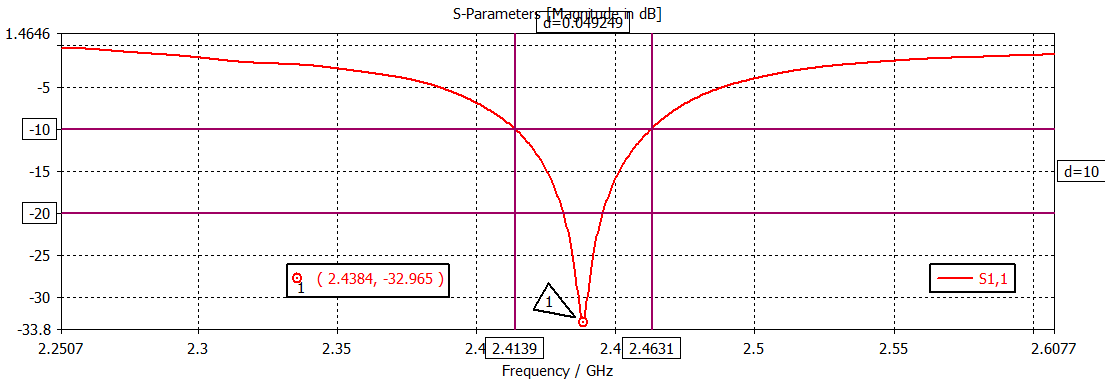
\includegraphics[scale=0.45]{p3_RL2}
	\caption{In-band view for the input reflection coefficient seen from full array input port.}
	\label{fig:p3_scattering_band}
\end{figure}

\begin{figure}[p] 
	\centering
	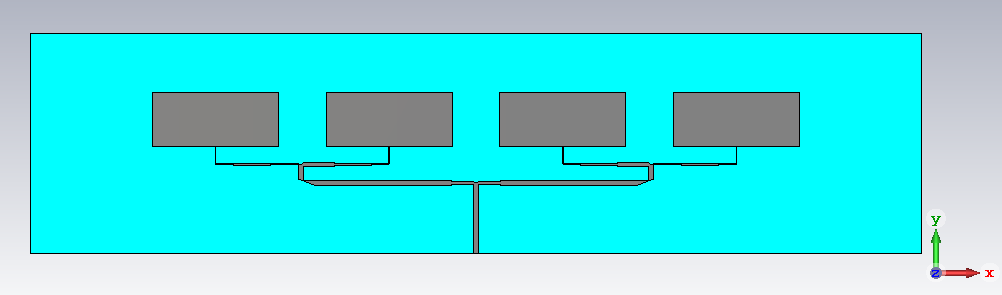
\includegraphics[scale=0.75, angle=90]{p3_array}
	\caption{Full array top view, (x,y) plane.}
	\label{fig:p3_array}
\end{figure}
\begin{figure}[p] 
	\centering
	\subfloat[][\emph{General settings}]{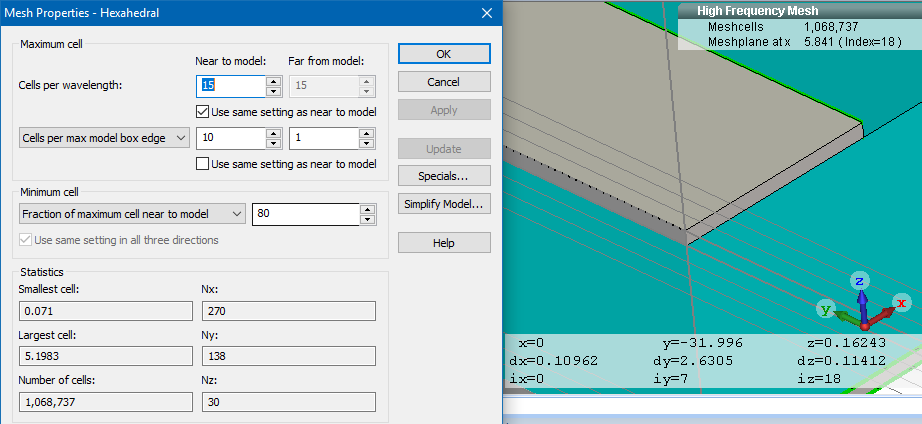
\includegraphics[scale=.5]{p3_mesh1}}\quad
	\subfloat[][\emph{Special settings}]{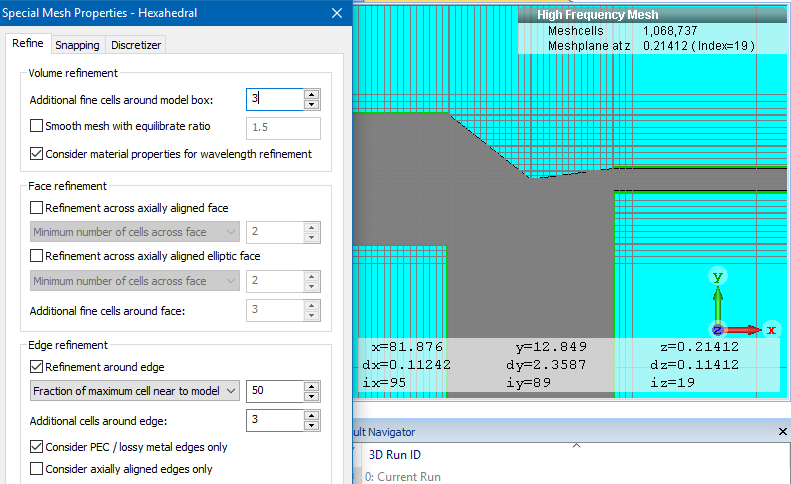
\includegraphics[scale=.5]{p3_mesh2}}\quad
	\subfloat[][\emph{Boundary conditions: symmetry plane}]{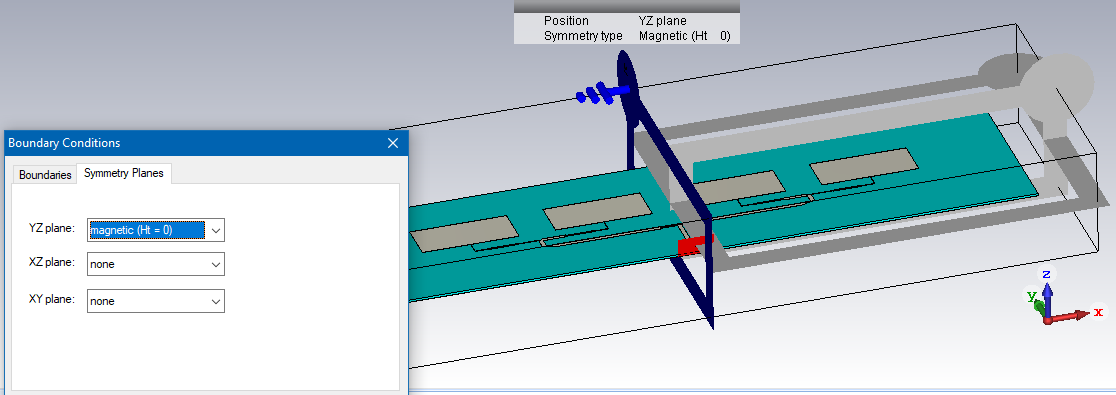
\includegraphics[scale=.4]{p3_JamesBonday}}\\
	\caption{Mesh general and special settings. As it appears the mesh has been increased to fit all the bends and narrower lines the best way.}.
	\label{fig:p3_mesh}
\end{figure}

\begin{figure}[p] 
	\centering
	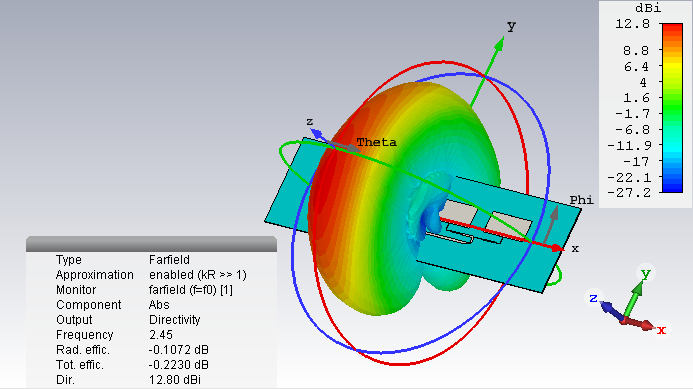
\includegraphics[scale=0.65]{p3_RP}
	\caption{3D far field radiation pattern.}
	\label{fig:p3_RP}
\end{figure}
\begin{figure}[p] 
	\centering
	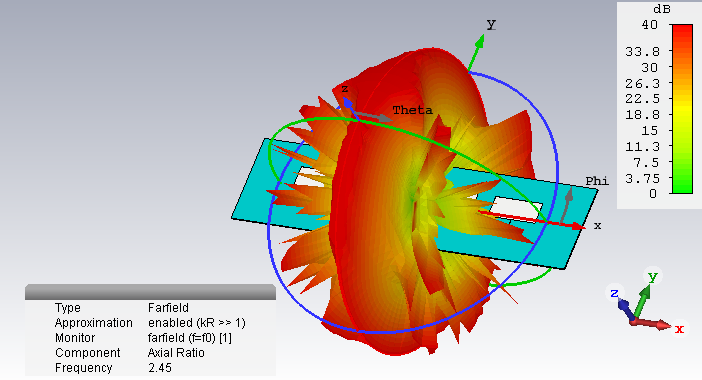
\includegraphics[scale=0.65]{p3_axial}
	\caption{Far field axial ratio.}
	\label{fig:p3_axial}
\end{figure}
\begin{figure}[p] 
	\centering
	\subfloat[][\emph{(x,y) plane cut, $\theta=0^\circ$}]{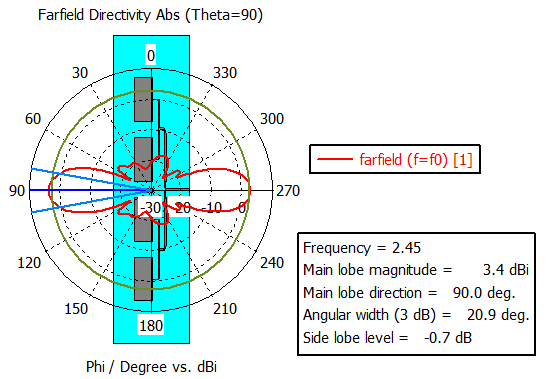
\includegraphics[scale=.7]{p3_XY}}\quad
	\subfloat[][\emph{(y,z) plane cut, $\varphi=0^\circ$}]{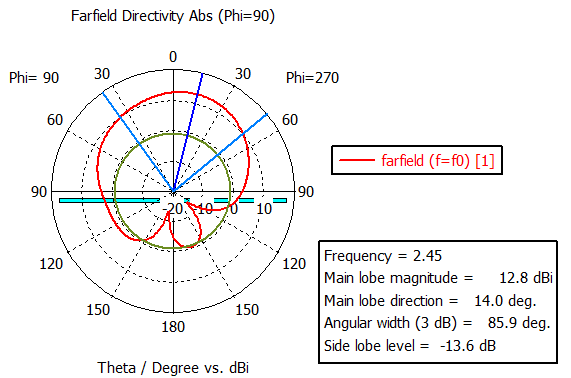
\includegraphics[scale=.7]{p3_YZ}}\\
	\caption{Radiation pattern's directivity polar cut planes. As it appears the array radiates broadside within the (y,z) plane. The radiation is minimum along the negative $y$-direction.}.
	\label{fig:p3_cuts1}
\end{figure}

\begin{figure}[p] 
	\centering
	\subfloat[][\emph{(x,z) plane polar cut,$\varphi=0^\circ$}]{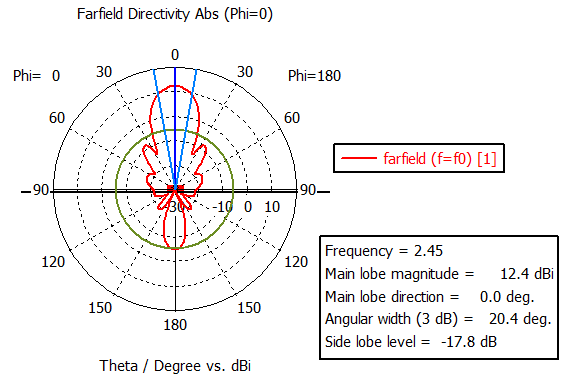
\includegraphics[scale=.7]{p3_XZ}}\quad
	\subfloat[][\emph{(x,z) plane cartesian view, $\varphi=0^\circ$}]{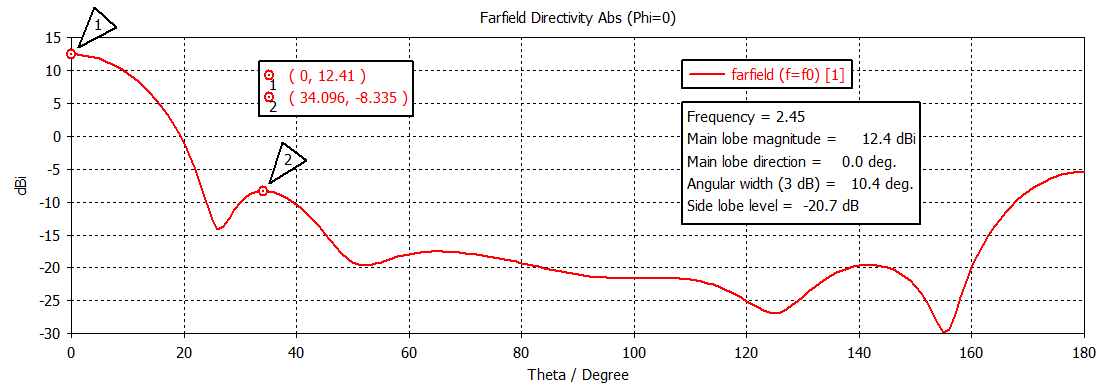
\includegraphics[scale=.4]{p3_XZ_cart}}\quad
		\subfloat[][\emph{positive (x,z) plane cartesian view, $\varphi=0^\circ$}]{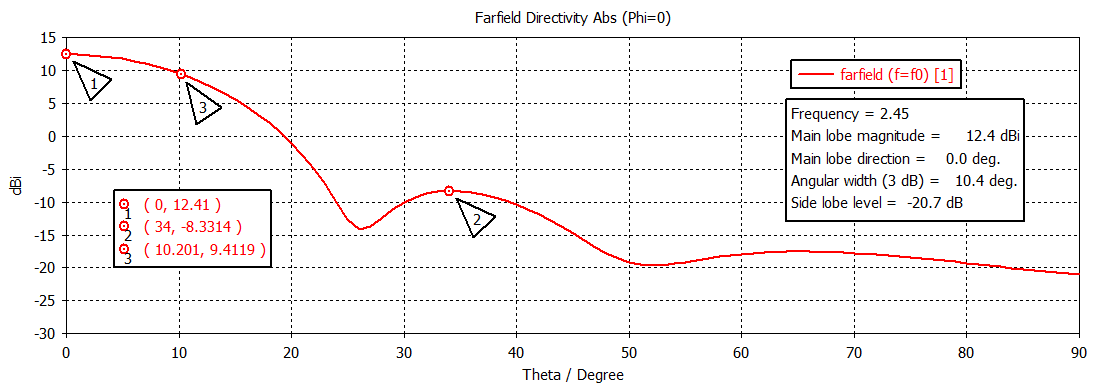
\includegraphics[scale=.4]{p3_XZ_cart2}}\\
	\caption{Radiation pattern's cut planes. As it appears the array radiates broadside within the (y,z) plane. The side lobes level limit is fulfilled, HPBW=20.4$^\circ$.}.
	\label{fig:p3_cuts2}
\end{figure}

\end{document}
